\documentclass[11pt]{sensys-proc}

\usepackage{graphicx}
\DeclareGraphicsExtensions{.pdf,.jpg,.png}
\graphicspath{{./figures/} {./plots/}}

\usepackage{balance}
\usepackage{comment}
\usepackage{xspace}
\usepackage[export]{adjustbox}
\usepackage{wrapfig}
\newcommand{\chain}{Chain\xspace}
\numberofauthors{3}

%\author{
%
% The command \alignauthor (no curly braces needed) should
% precede each author name, affiliation/snail-mail address and
% e-mail address. Additionally, tag each line of
% affiliation/address with \affaddr, and tag the
%% e-mail address with \email.
%\alignauthor Alice Security \\
%        \affaddr{Department of Computer Science}\\
%        \affaddr{University of Southern California}\\
%       \email{alice@example.edu}
%\alignauthor Bob Privacy \\
%    \affaddr{Networked Embedded Systems Group}\\
%    \affaddr{Swedish Institute of Computer Science}\\
%    \email{bob@example.se}
%}

\title{TAPIR: Threaded Application Programming on Intermittant Resources}

\begin{document}

\maketitle

%Only including an abstract since it looks like the submission site wants one...
\begin{abstract}
Killer abstract.
\end{abstract}

\section{Introduction/Background}
  \label{sec:intro}
  Chain, DINO\\
  Multithreading\\
  Intermittance Review\\
  RMW\\
  Example Citation\cite{RC,Grace}!


%Sample of adding a picture across the top of a split page...
\begin{figure*}
\centering
\begin{minipage}[b]{0.49\textwidth}
  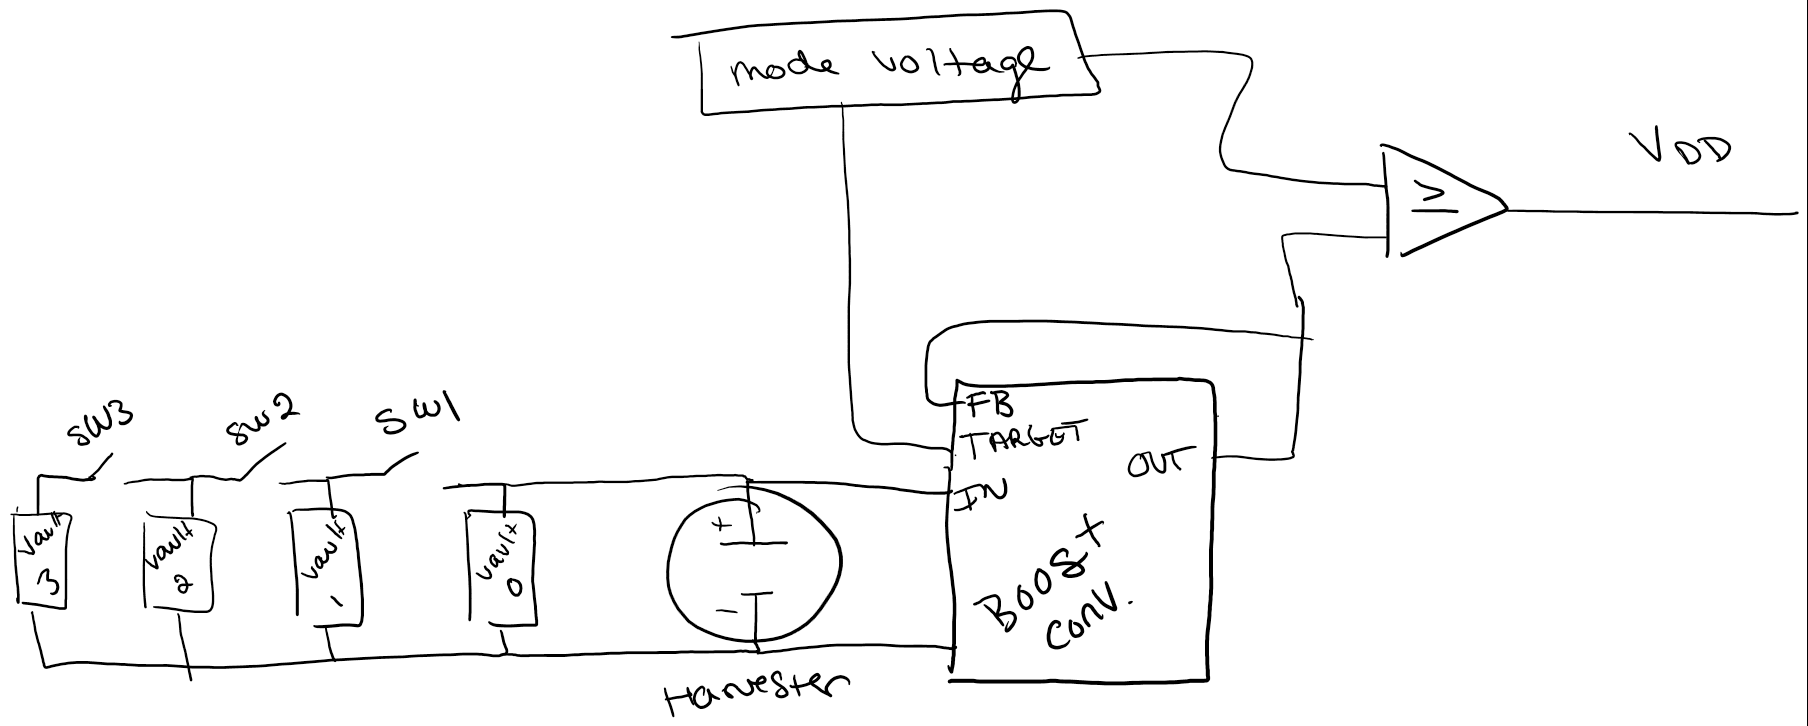
\includegraphics[width=0.95\textwidth,center]{capybara-all.png}
\caption{Capybara power system overview}\label{label-a}
\end{minipage}\hfill
\begin{minipage}[b]{0.49\textwidth}
  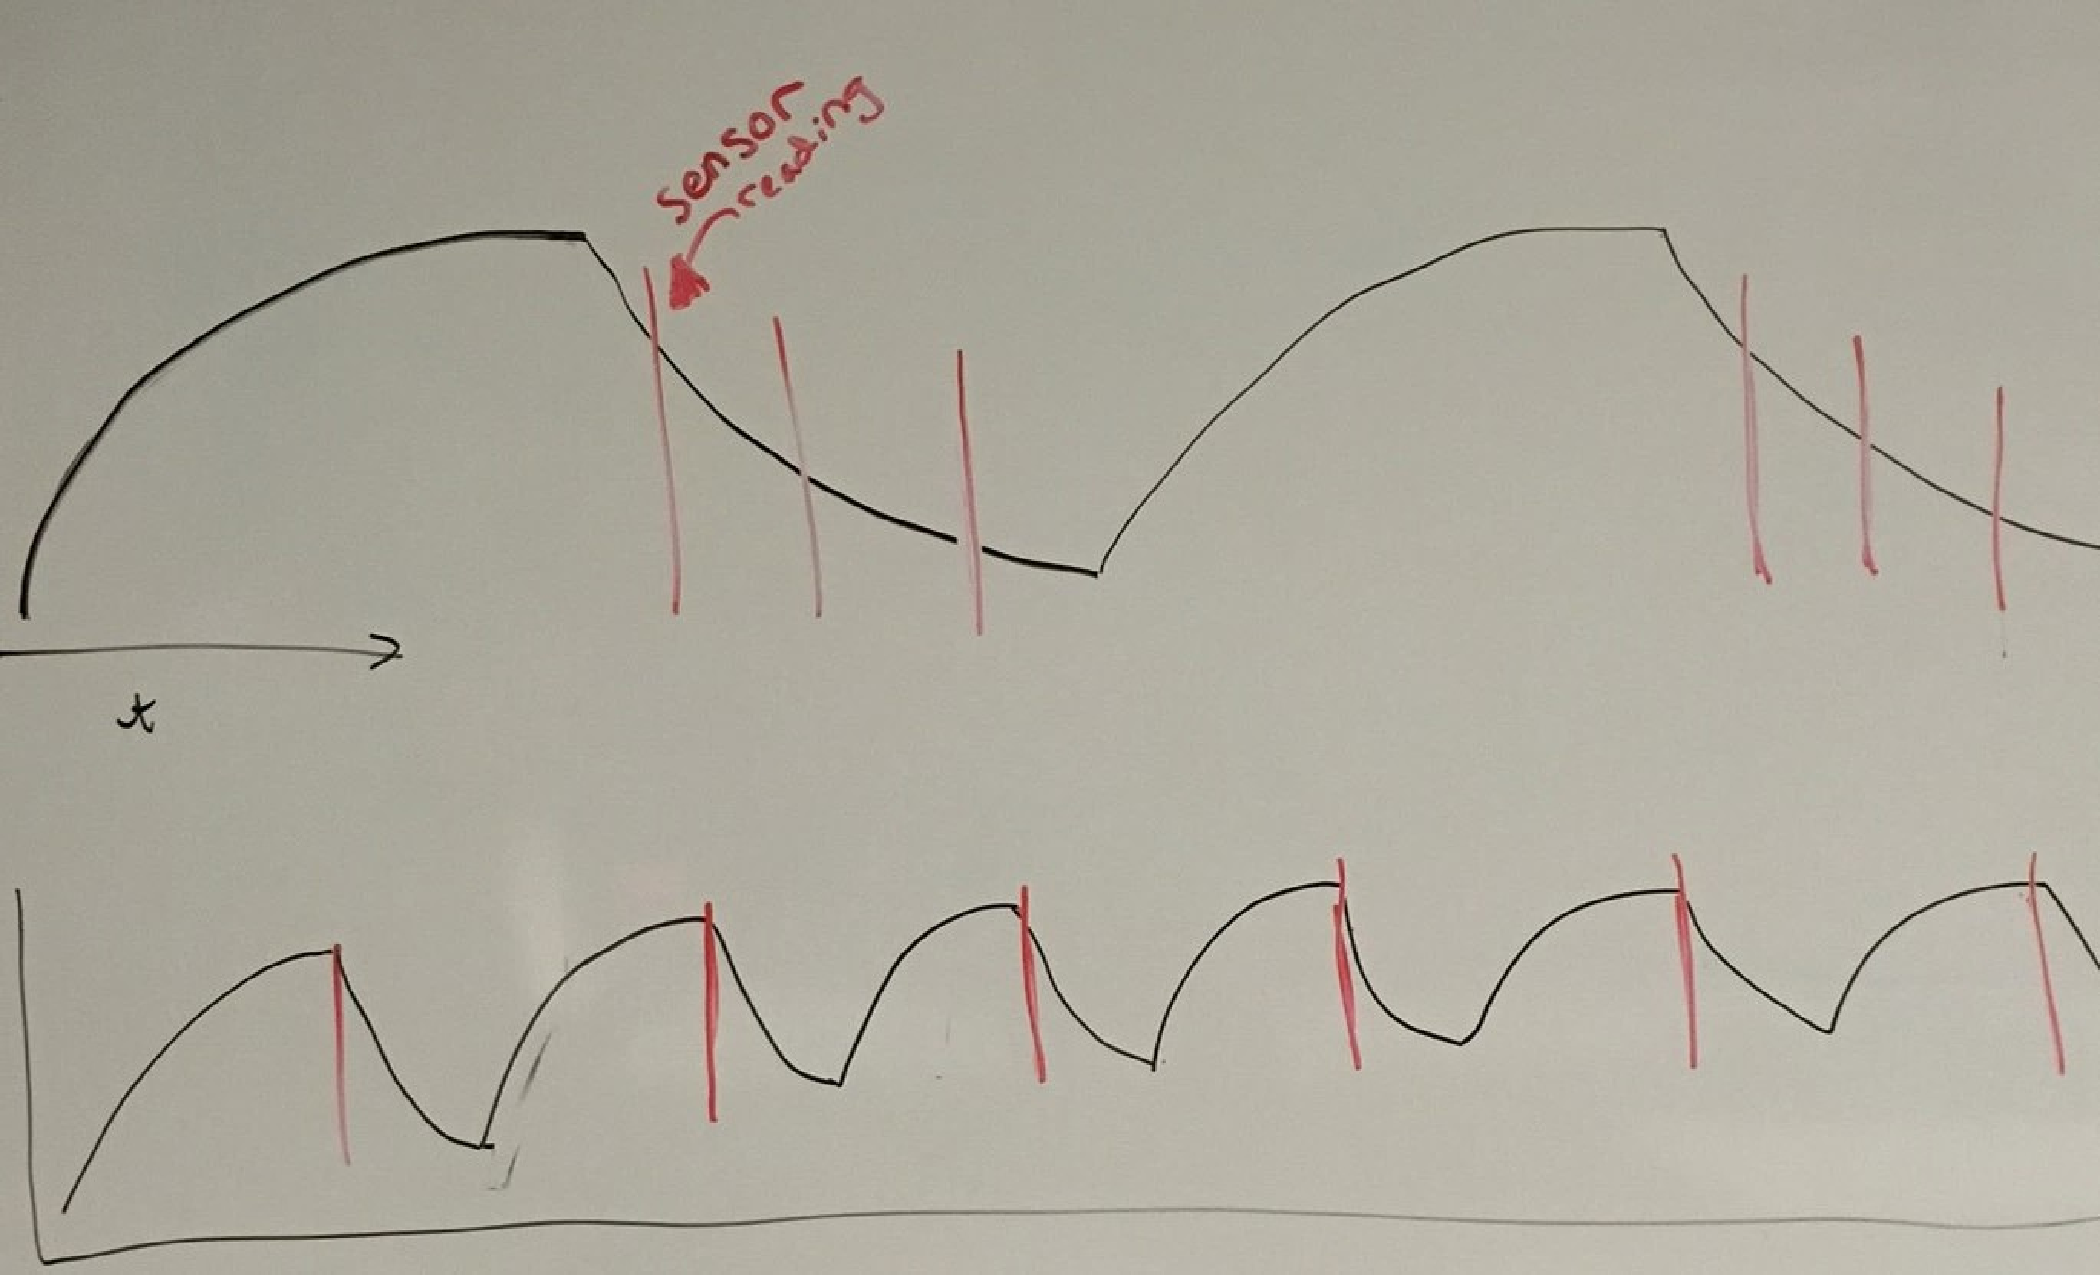
\includegraphics[width=0.95\textwidth,center]{power_modes.pdf}
\caption{Effect of different power modes}\label{label-b}
\end{minipage}
\end{figure*}

More text after the picture to show how that looks...


\section{Related Work}
Operating system work\\
TU delft guys...\\
Energy Align\\


\section{Chain Discussion}
Arrays in channels and why that's bad\\
MAX\_NUM\_DIRTY\_FIELDS\\
Explioting the fact that there isn't a compiler\\


\section{What we did} % TODO change title
Scheduler\\
Interrupts\\
Mutexes\\
User programming model for threads\\
Interrupts\\
Round Robin (alternatives, on reboot)\\
SIMD vs MIMD\\
SIMD w/ channels (you don't get your own registers...etc -
    just channels, since intermittant)\\


\section{Implementation}
We only had to break \chain a little. We promise!
Scheduler Data structures and idempotence (what we broke and why we broke it)\\
Mutexes (Simple, meant for pseudo channels)\\
Interrupts (mucked with IE flags)\\


\section{Results}
No really, there will be things here!
Applications/measurements\\
Blinker (x2)\\
RSA+cukoo\\
No verification\\
Memory overhead (read off compiliation)\\
Performance (\# reboots)\\


\section{Future Work}
Duplicating channels (a little renaming or sharing arrays with mutexes)\\
Optimizations to reduce overhead\\


\section{Conclusion}
Multithreading in intermittence {\em is} a good idea!


\balance
\bibliographystyle{abbrv}
\bibliography{sigproc}  % sigproc.bib is the name of the Bibliography in this case
\end{document}
